\documentclass[a4paper,12pt]{article}
\usepackage[utf8]{inputenc}

\usepackage[utf8]{inputenc}
\usepackage[T2A]{fontenc}
\usepackage[english,russian]{babel}
\usepackage{amsthm}
\usepackage{amsmath}
\usepackage{amssymb}
\usepackage{tikz}
\usepackage{textcomp}
\usepackage{marvosym}
\usepackage{ esint }
\usepackage{mathtext}
\usepackage{siunitx} % Required for alignment
\usepackage{subfigure}
\usepackage{multirow}
\usepackage{rotating}
\usepackage{afterpage}
\usepackage[arrowdel]{physics}
\usepackage{booktabs}
\setlength{\topmargin}{-0.5in}
\setlength{\textheight}{9.1in}
\setlength{\oddsidemargin}{-0.4in}
\setlength{\evensidemargin}{-0.4in}
\setlength{\textwidth}{7in}
\setlength{\parindent}{0ex}
\setlength{\parskip}{1ex}
\newcommand{\ndiv}{\hspace{-4pt}\not|\hspace{2pt}}
\usepackage{graphicx}
\usepackage{float}
\usepackage{wrapfig}
\usepackage{pgfplots}
\usepackage{caption}
\pgfplotsset{compat=1.16}
\graphicspath{ {./images/} }
\usepackage{graphicx}
\RequirePackage{caption}
\DeclareCaptionLabelSeparator{defffis}{ — }
\captionsetup{justification=centering,labelsep=defffis}
\usepackage{caption} \captionsetup[table]{labelsep=endash,justification=justified,singlelinecheck=false,font=normalsize}
\usepackage{amsfonts,mathtools}

\title{Лабораторная работа № 4.3.1\\ Изучение дифракции света}
\author{Илья Прамский}
\date{Февраль 2024}

\begin{document}

\maketitle
\newpage

\textbf{Цель работы:} исследовать явления дифракции Френеля и Фраунгофера на щели, изучить влияние дифракции на разрешающую способность оптических инструментов.


\textbf{В работе используются:} оптическая скамья, ртутная лампа, мо- нохроматор, щели с регулируемой шириной, рамка с вертикальной нитью, двойная щель, микроскоп на поперечных салазках с микро- метрическим винтом, зрительная труба.

\section{Теоретическая справка}
\subsection{Дифракция Френеля на щели}

Схема установки для наблюдения дифракции Френеля на щели представлена на рис. \ref{labA}. Световые лучи освещают щель $ S_2 $ и испытывают на ней дифракцию. Дифракционная картина рассматривается с помощью микроскопа М, сфокусированного на некоторую плоскость наблюдения П.

\begin{figure}[H]
	\centering
	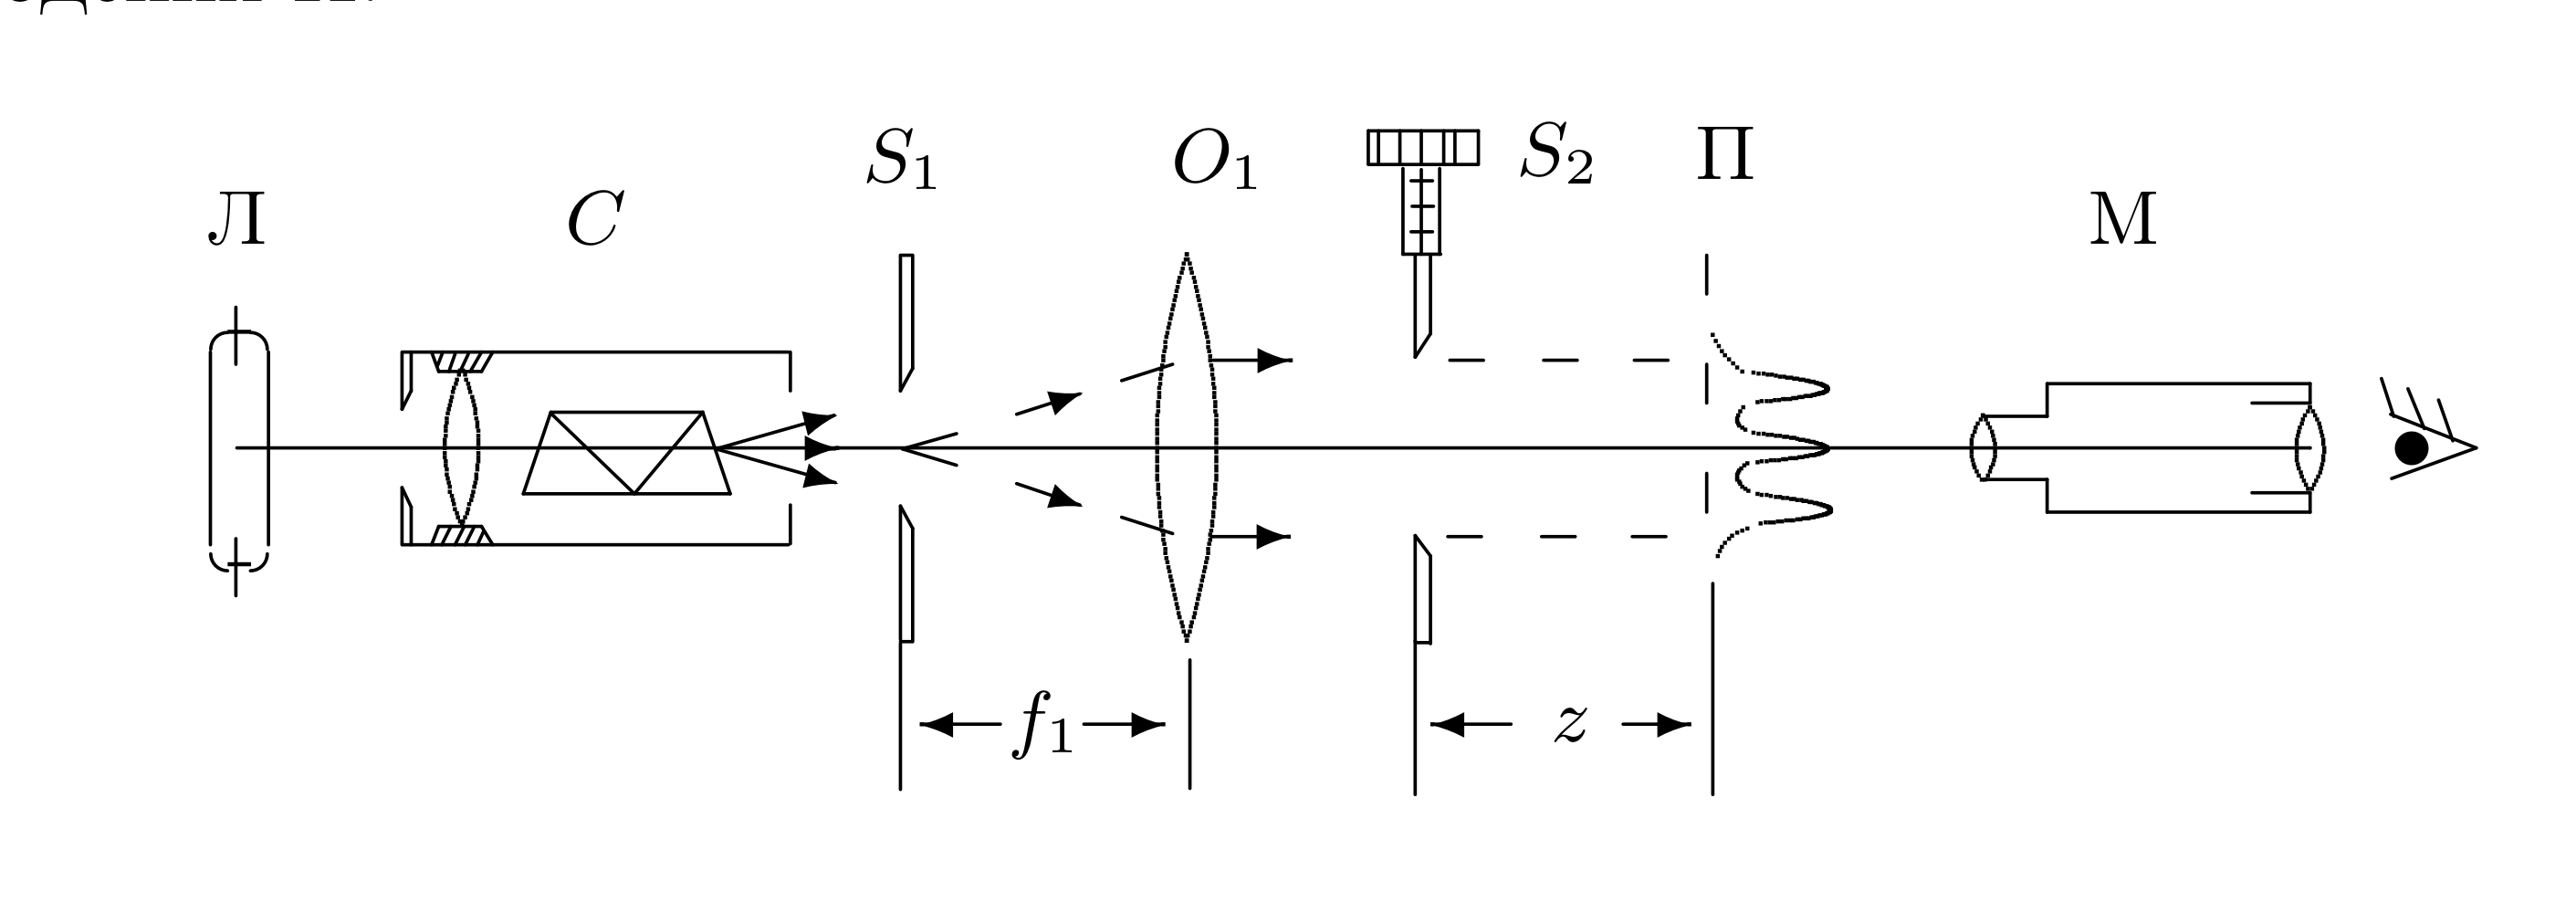
\includegraphics[scale=0.15]{alab.jpeg}
	\caption{Схема установки для наблюдения дифракции Френеля}
	\label{labA}
\end{figure}

Щель $ S_2 $ освещается параллельным пучком монохроматического света с помощью коллиматора, образованного объективом $ O_1 $, и щелью $S_1$, 
находящейся в его фокусе. На щель $ S_1 $ сфокусировано изображение спектральной линии, выделенной из спектра ртутной лампы Л 
при помощи простого монохроматора C, в котором используется призма прямого зрения. 
Распределение интенсивности света в плоскости наблюдения П проще всего рассчитывать с помощью зон Френеля 
(для щели их иногда называют зонами Шустера). При освещении щели $ S_2 $ параллельным пучком лучей (плоская волна) 
зоны Френеля представляют собой полоски, параллельные краям щели (рис. \ref{zone}). 
Результирующая амплитуда в точке наблюдения определяется суперпозицией колебаний от тех зон Френеля, 
которые не перекрыты створками щели. Графическое определение результирующей амплитуды производится с помощью векторной диаграммы --- спирали Корню. 
Суммарная ширина $ n $ зон Френеля (Шустера) определяется соотношением:

\begin{equation}\label{xin}
\xi_m = \sqrt{zn\lambda}
\end{equation}
где $ z $ --- расстояние от щели до плоскости наблюдения (рис. \ref{labA}), а $ \lambda $ --- длина волны.

\begin{figure}[H]
	\begin{center}
		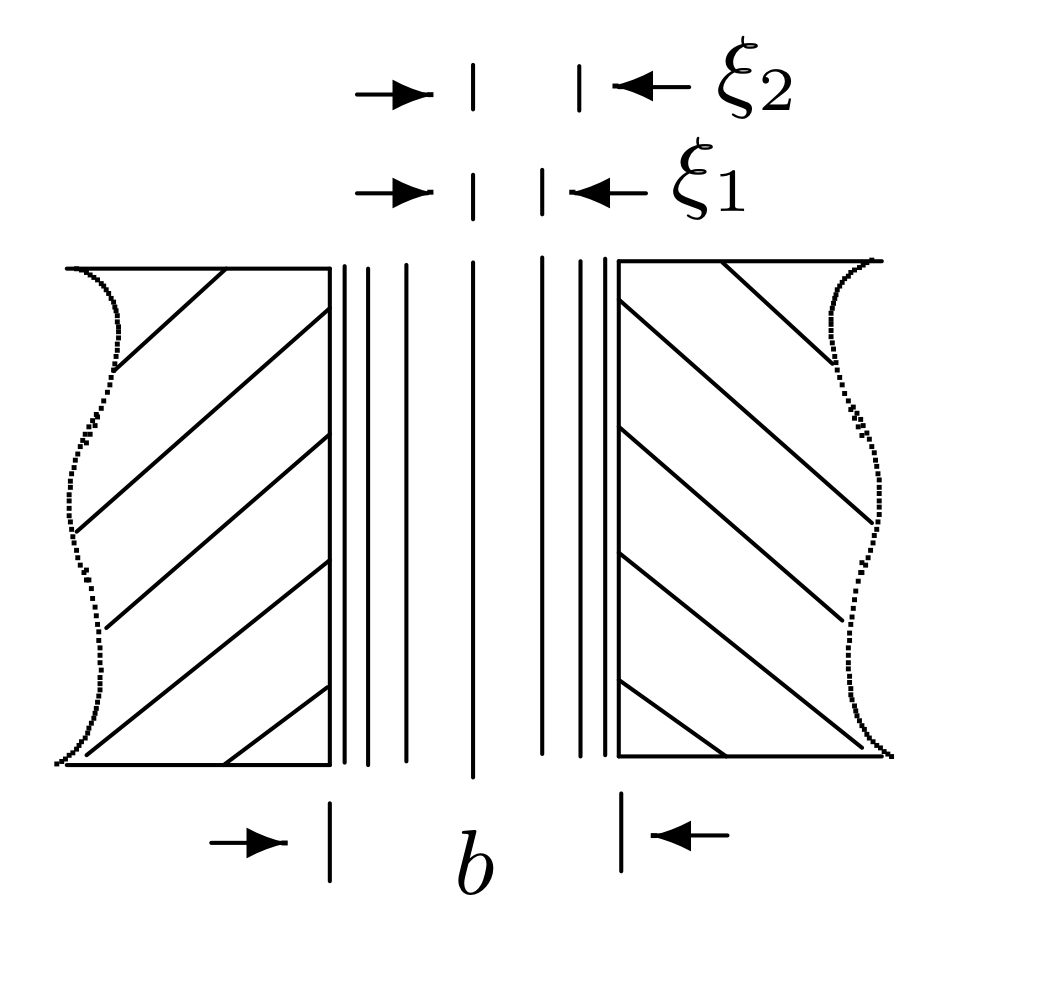
\includegraphics[scale=0.15]{zone.jpeg}
	\end{center}
	\caption{Зоны Френеля}
	\label{zone}
\end{figure}

Вид наблюдаемой дифракционной картины
на щели шириной $ b $ определяется волновым параметром $ p $ или числом Френеля $ C $ (число открытых полных зон):


\begin{equation}\label{p}
p = \dfrac{\sqrt{z \lambda}}{b}, \qquad C = \dfrac{1}{p^2}
\end{equation}




\subsection{Дифракция Фраунгофера на одной щели}

На значительном удалении от щели, когда выполнено условие $ C \ll 1 $
(то есть ширина щели становится значительно меньше ширины первой
зоны Френеля, $ b \ll \sqrt{\lambda z} $), изображение щели размывается и возникает
дифракционная картина, называемая дифракцией Фраунгофера.

Дифракцию Френеля и Фраунгофера можно наблюдать на одной
и той же установке (рис. \ref{labA}). Однако при обычных размерах установки дифракция Фраунгофера возникает только при очень узких щелях.

\begin{figure}[H]
	\centering
	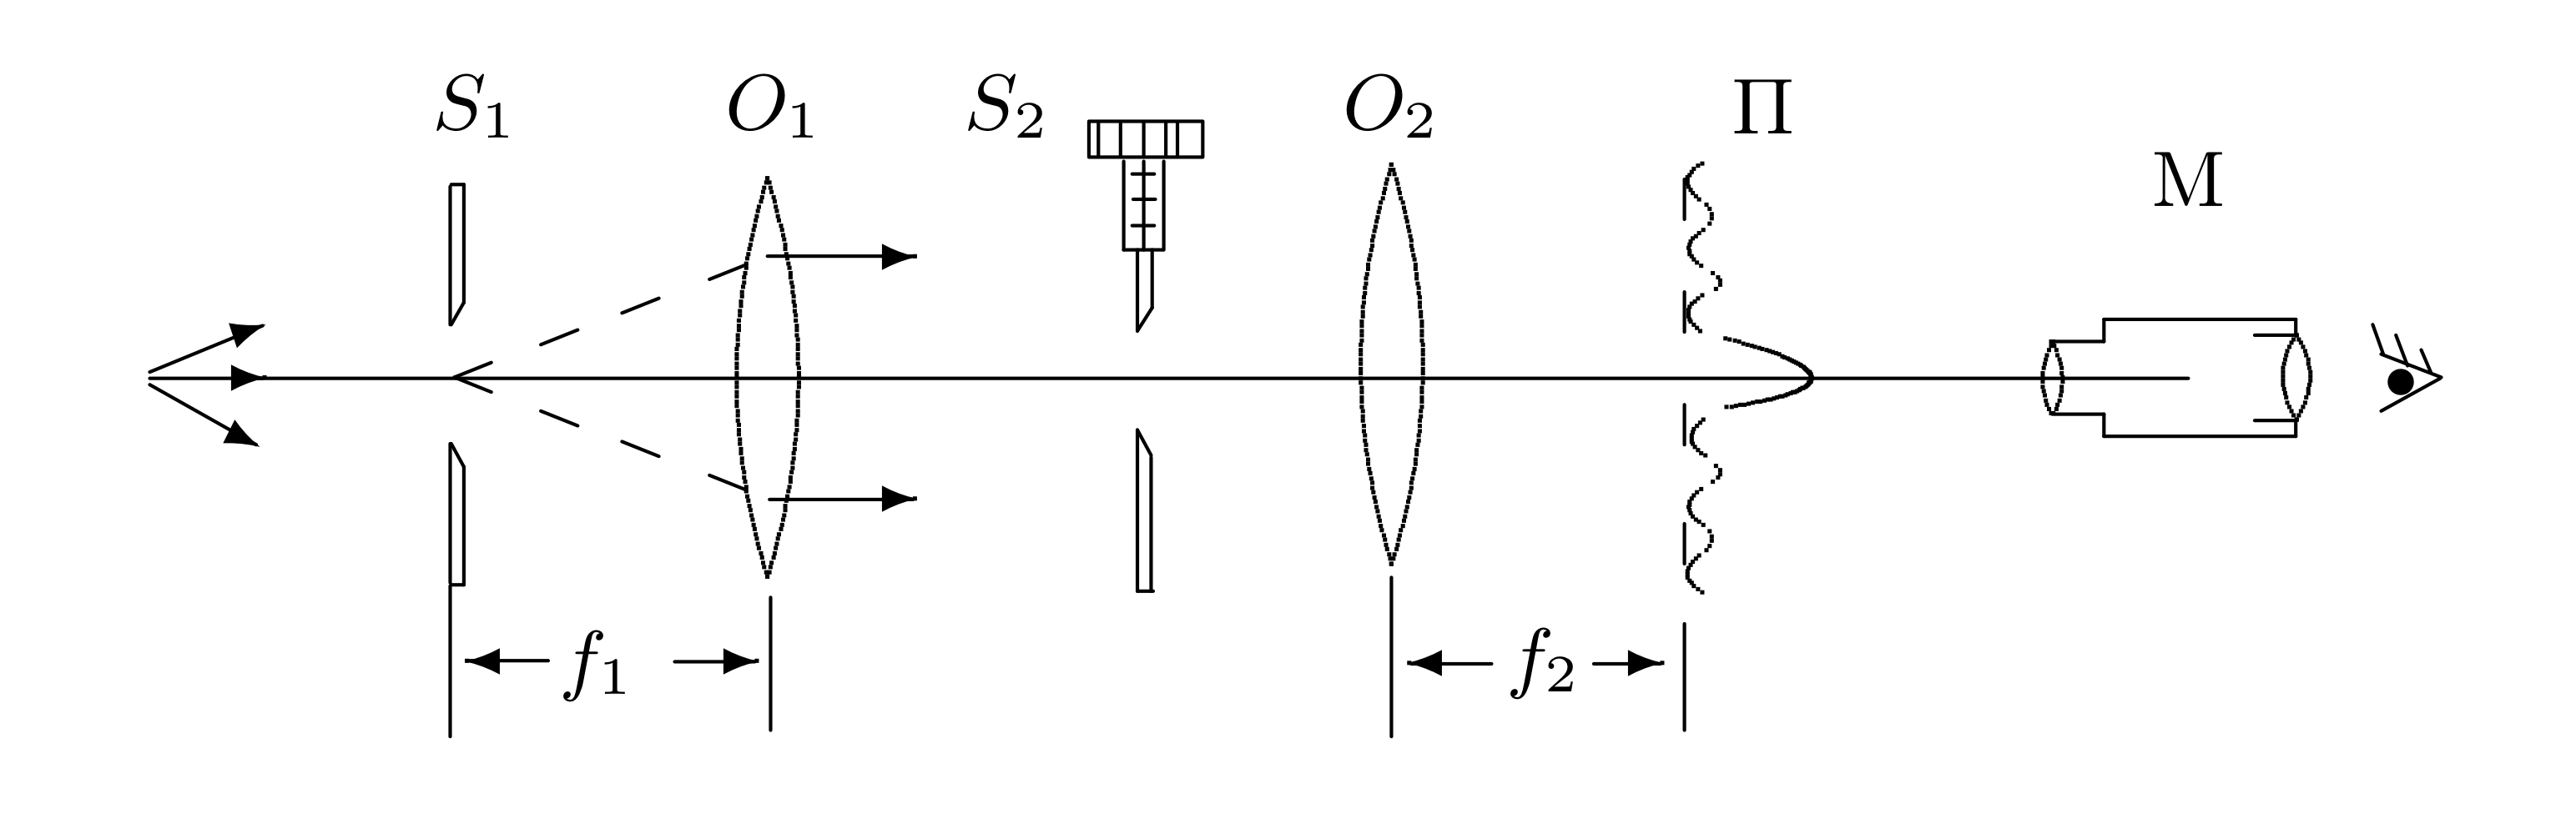
\includegraphics[scale=0.15]{blab.jpeg}
	\caption{Схема установки для наблюдения дифракции Фраунгофера на щели}
	\label{labB}
\end{figure}

Например, при $ z \approx  20-40 $  см и $  \lambda \approx 5 \cdot 10^{-5}  $   см получаем $  b \ll 0,3 $ мм. Поскольку работать с такими тонкими щелями неудобно, для наблюдения дифракции Фраунгофера к схеме, изображённой на рис. \ref{labA}, добавляется объектив $ O_2  $ (рис. \ref{labB}).

Дифракционная картина наблюдается здесь в фокальной плоскости
объектива $ O_2 $. Каждому значению угла $ \theta $ соответствует в этой плоскости точка, отстоящая от оптической оси на расстоянии

\begin{equation}\label{x}
x = f_2 \tg \theta \approx f_2 \theta
\end{equation}


плоскости наблюдается неискаженная дифракционная картина Фраунгофера. Эта картина соответствует бесконечно удалённой плоскости
наблюдения.

В центре поля зрения наблюдается дифракционный максимум (светлая полоса). При малых углах $ \theta $ положение минимумов (тёмных полос)
определяется, соотношением

\begin{equation}\label{theta_m}
\theta_m = m \dfrac{\lambda}{b}
\end{equation}

Расстояние $ x_m $ от тёмной полосы до оптической оси объектива $ O_2 $ пропорционально фокусному расстоянию $ f_2 $. Из \eqref{x} и \eqref{theta_m} следует 

\begin{equation}\label{xm}
x_m = m \dfrac{\lambda}{b} f_2
\end{equation}

Видно, что при малых углах минимумы эквидистантны, а расстояния $ \delta x $ между минимумами обратно пропорциональны ширине $ b $ щели $ S_2 $.



\subsection{Дифракция Фраунгофера на двух щелях}

Для наблюдения дифракции Фраунгофера на двух щелях в установке (рис. \ref{labB}) следует заменить щель $ S_2 $ экраном Э с двумя щелями
(рис. \ref{labC}). При этом для оценки влияния ширины входной щели на чёткость дифракционной картины вместо входной щели $ S_1 $ следует поставить щель с микрометрическим винтом. Два дифракционных изображения входной щели, одно из которых образовано лучами, прошедшими через левую, а другое --- через правую щели, накладываются друг на друга.

\begin{figure}[H]
	\centering
	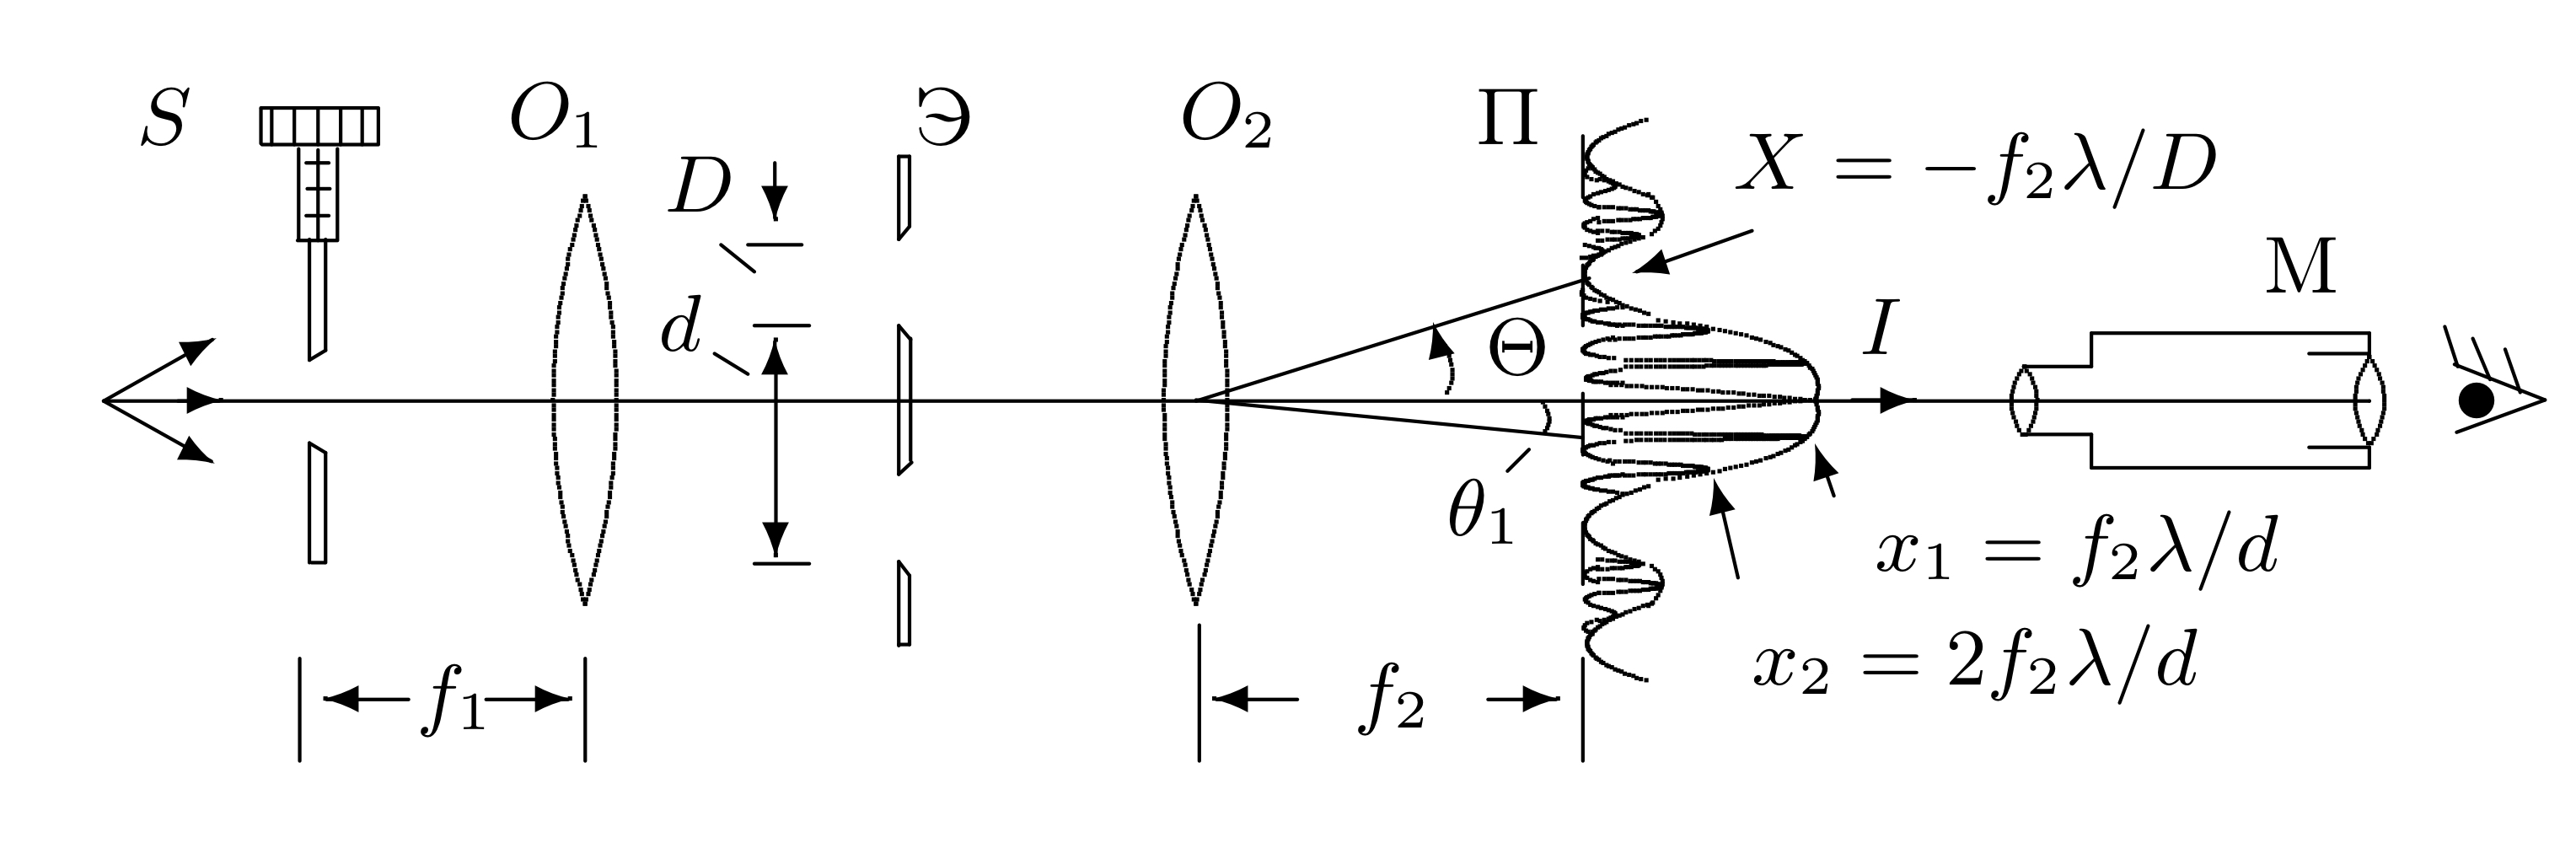
\includegraphics[scale=0.15]{clab.jpeg}
	\caption{Схема установки для наблюдения дифракции Фраунгофера на двух щелях}
	\label{labC}
\end{figure}

Если входная щель достаточно узка, то дифракционная картина
в плоскости П (рис. \ref{labC}) подобна той, что получалась при дифракции
на одной щели (рис. \ref{labB}), однако теперь вся картина испещрена рядом
дополнительных узких полос.
Угловая координата $ \theta_m $ интерференционного максимума $ m $-го порядка определяется соотношением

\begin{equation}\label{}
\theta_m = m \dfrac{\lambda}{b}
\end{equation}

где $ d $ --- расстояние между щелями. Линейное расстояние $ \delta x $ между соседними интерференционными полосами в плоскости П равно, поэтому

\begin{equation}\label{dx}
\delta x = f_2 \dfrac{\lambda}{d}
\end{equation}

На рис. \ref{labC} показано распределение интенсивности в фокальной плоскости объектива $ O_2 $. Штриховой линией (в увеличенном масштабе)
изображено распределение интенсивности при дифракции света на одиночной щели. Нетрудно оценить число n интерференционных полос,
укладывающихся в области центрального дифракционного максимума.
Согласно \eqref{xm} полная ширина главного максимума равна $ 2 f_2 \lambda /b $, где $ b $ ширина щели, отсюда

\begin{equation}\label{n}
n = \dfrac{2f_2 \lambda}{b} \dfrac{1}{\delta x} = \dfrac{2d}{b}
\end{equation}

При дифракции света на двух щелях чёткая система интерференционных полос наблюдается только при достаточно узкой ширине входной щели $ S $, которую можно рассматривать как протяжённый источник света размером $ b $. Для наблюдения интерференции необходимо, чтобы расстояние $ d $между щелями не превышало радиуса когерентности

\begin{equation}\label{}
d \ll \dfrac{\lambda}{b} f_1
\end{equation}

Здесь $ b $ --- ширина входной щели $ S $ и, следовательно, $  b/f_1 $ --- её угловая ширина. Таким образом, по размытию интерференционной картины можно оценить размер источника. Этот метод используется в звёздном интерферометре при измерении угловых размеров звёзд.

\subsection{Влияние дифракции на разрешающую способность оптического инструмента}

Установка, представленная на рис. \ref{labB}, позволяет исследовать влияние дифракции на разрешающую способность оптических инструментов.

Как уже было выяснено, линзы $O_1$ и $ O_2$ в отсутствие щели $S_2$ создают в плоскости П изображение щели $S_1$, и это изображение рассматривается в микроскоп М. Таким образом, нашу установку можно рассматривать как оптический инструмент, предназначенный для получения изображения предмета. При этом коллиматор (щель $S_1$ и объектив $O_1$) является моделью далёкого предмета, а объектив $O_2$ и микроскоп М составляют зрительную трубу, наведённую на этот предмет.
Щель $S_2$, установленная непосредственно перед объективом $O_2$, позволяет изменять эффективный размер объектива и, следовательно, разрешающую способность оптической системы.

\begin{figure}[H]
	\centering
	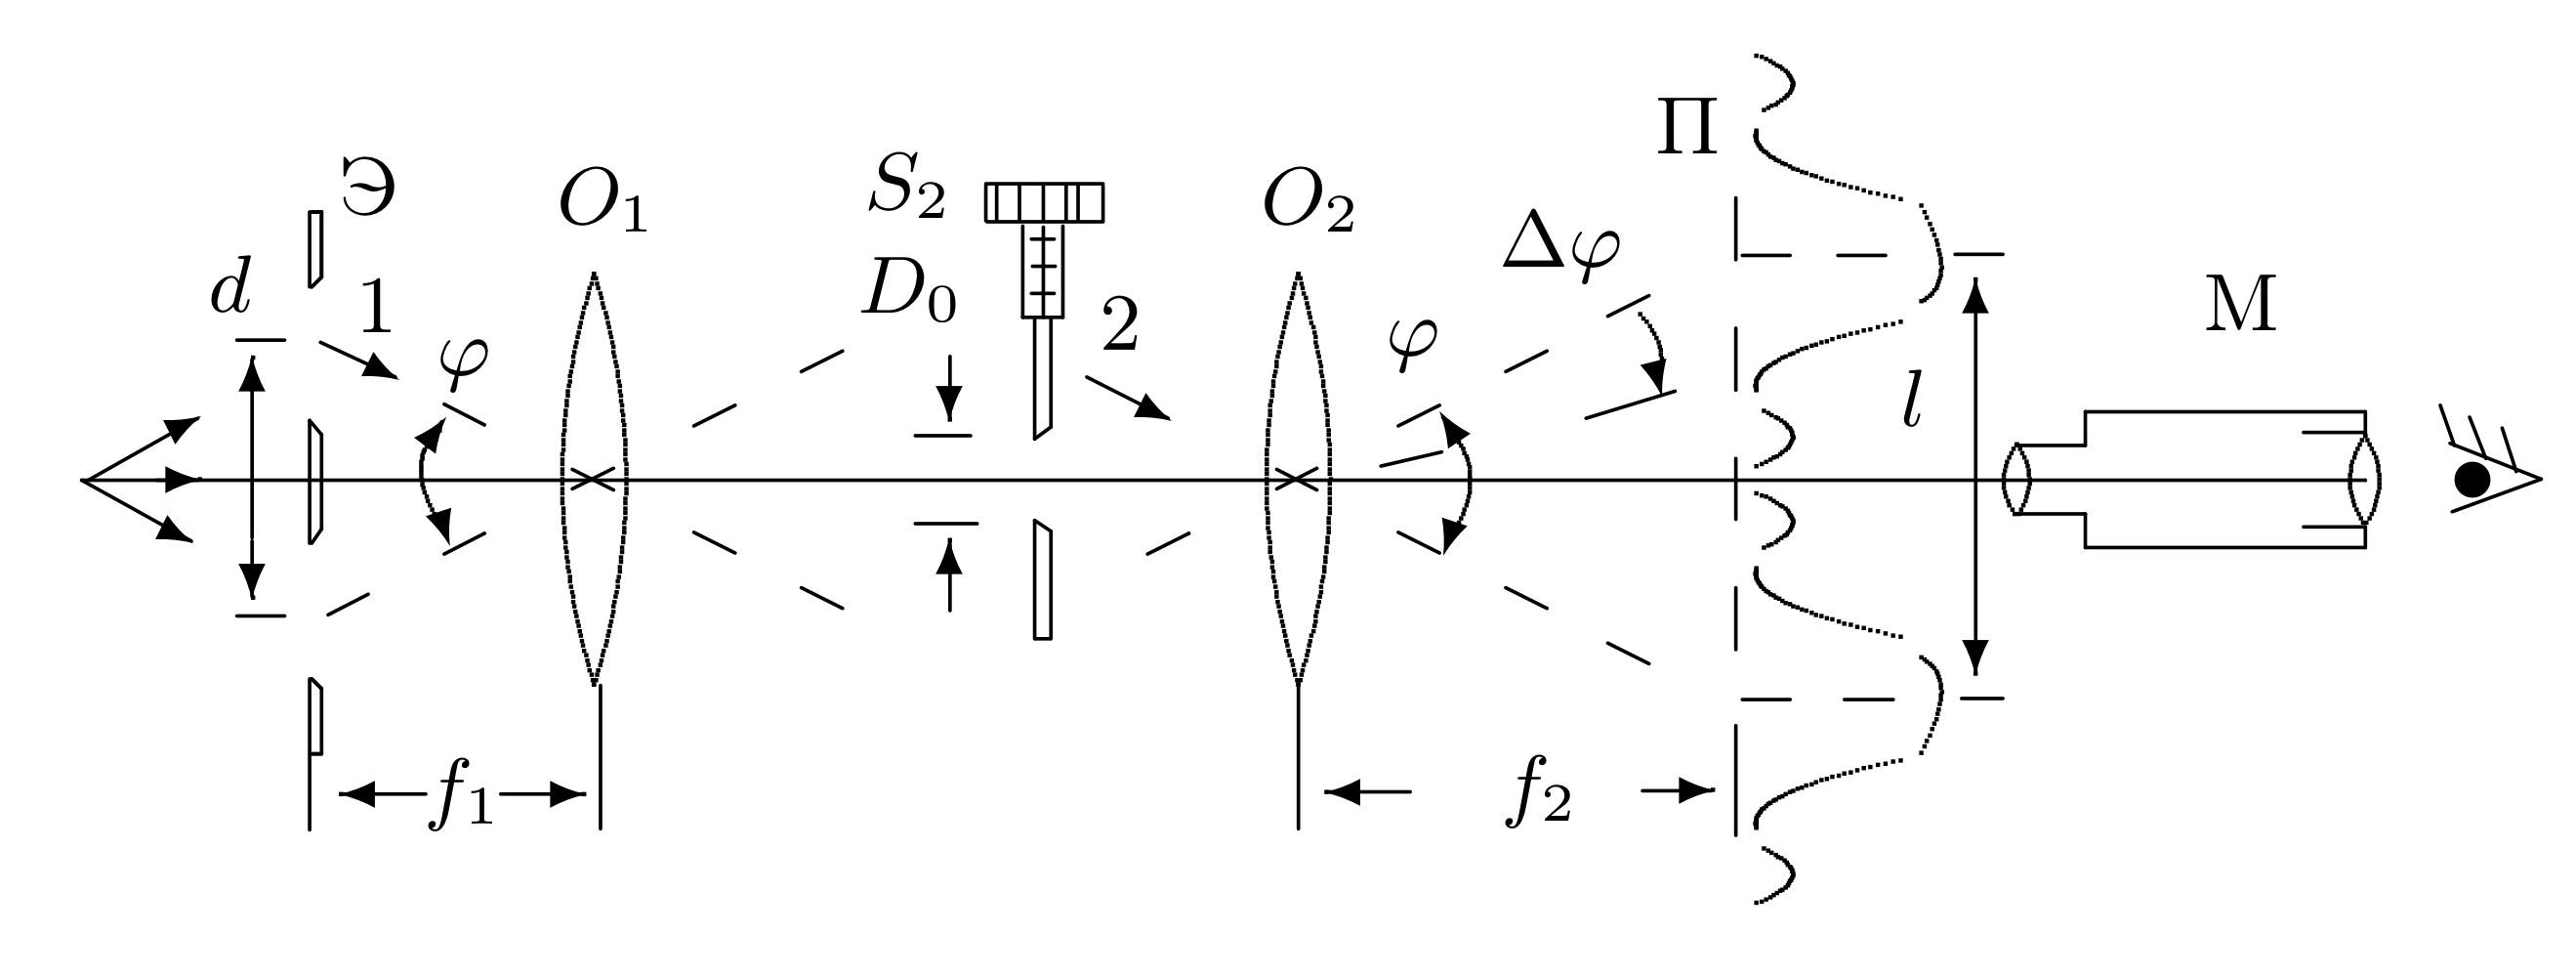
\includegraphics[scale=0.15]{dlab.jpeg}
	\caption{Схема установки для исследования разрешающей
		способности оптического инструмента}
	\label{labG}
\end{figure}

Поместим вместо щели $S_1$ экран Э с двумя узкими щелями, расстояние между которыми равно $d$ (рис. \ref{labG}). Тогда расстояние $l$ между изображениями щелей в плоскости П равно
\begin{equation}
l = \varphi f_2 = d \dfrac{f_2}{f_1},
\end{equation}
а ширина каждого изображения
\begin{equation}
\delta x \approx \dfrac{\lambda}{b} f_2
\end{equation}
определяется дифракцией света на щели $S_2$. Когда полуширина дифракционного изображения превышает расстояние между изображениями, то по виду дифракционной картины трудно определить, представляет собой источник двойную или одиночную щель.

Условия, при которых ещё можно различить, имеем мы дело с одной или двумя щелями, для разных наблюдателей различны. Для того чтобы исключить связанный с этим произвол, пользуются обычно критерием Рэлея, который приблизительно соответствует возможностям визуального наблюдения: изображения считаются различимыми, когда максимум одного дифракционного пятна совпадает с минимумом другого, а в условиях нашей задачи --- когда полуширина дифракционного изображения $\delta x$ совпадает с расстоянием $l$ между изображениями отдельных щелей:
\begin{equation}
\delta x \sim l \to \dfrac{\lambda}{b} \sim \dfrac{d}{f_1}.
\end{equation}

\section{Ход работы}
\subsection{Дифракция Френеля на щели}
Соберём установку согласно рисунку $1$, далее настроим её согласно методическим материалам так, чтобы в микроскоп наблюдалась дифракция Френеля.

Наибольшая чёткость картины достигается при $L = 62,00 \pm 0,14$ см(координата по шкале на продольной скамье). В дальнейшем разница между значением этой координаты и координаты, при которой наблюдаем дифракцию, будет давать нам величину z - расстояние от щели до плоскости наблюдения.

Теперь будем отодвигать микроскоп от установки и фиксировать зависимость координаты микроскопа от числа n наблюдаемых полос. Также найдём значение $2\xi_n$ по формуле (\ref{xin}). При этом длина волны зелёной линии ртути равна $\lambda = 5461 А = 54,61 \cdot 10^{-6}$ см. Также учтём, что зон Шустера на одну больше, чем тёмных полос($n$ в формуле (\ref{xin}) - количество зон Френеля). Погрешность измерения x равна $\sigma_x = 0,14$ см(т.к. погрешность на шкале продольной скамьи и на шкале тубуса).

\begin{table}[H]
    \centering
    \begin{tabular}{ccccc}
      m  & x, см  & z, см & 2$\xi_n$, мкм & $\sigma_{\xi_n}$, мкм\\
      1   & 59,20 & 2,80  & 247,3 & 9 \\
      2   & 60,00 & 2,00  & 295,6 & 14\\
      3   & 60,60 & 1,40  & 302,9 & 21\\
      4   & 60,95 & 1,05  & 302,9 & 30\\
      5   & 61,05 & 0,95  & 322,1 & 34\\
    \end{tabular}
    \label{tab:my_label}
\end{table}
Также измерим значение щели при помощи микрометрического винта и поперечных салазок микроскопа. Получилось $b_1 = 365 \pm 10$ мкм и $b_2 = 340 \pm 20$ мкм. Теперь построим график зависимости $2\xi_n = f(n)$ и отложим на нём величину $b_1$. Как видно из графика, все значения лежат рядом со значением диаметра, измеренным при помощи микрометрического винта. На самом деле должно был получиться график из точек, которые при увеличении n всё ближе располагаются к значению $b_1$. Но данное несходство можно объяснить тем, что определить точный момент появления новых полос очень затруднительно, из-за чего и возникает такая ошибка.


\begin{figure}[H]
	\centering
	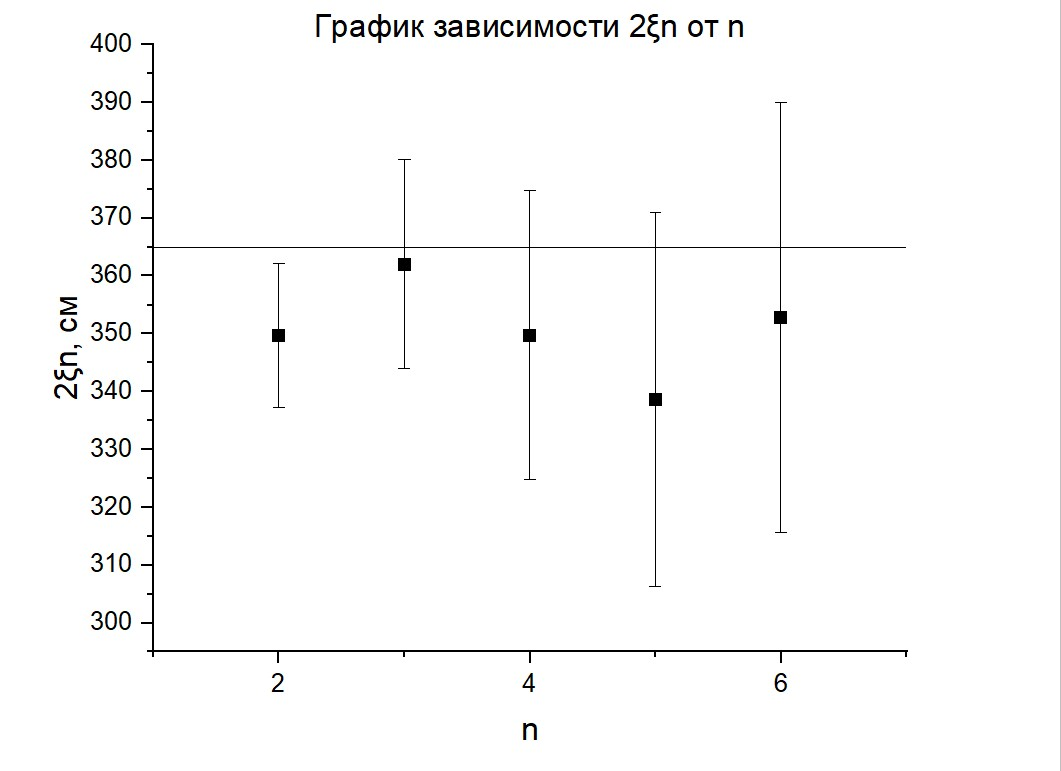
\includegraphics[scale=0.75]{graph1.jpg}
	\label{graph1}
\end{figure}

\subsection{Качественные наблюдения}
При уменьшении щели уменьшается количество дифракционных 
полос. Это согласуется с теорией и обусловлено возрастанием 
волнового параметра (\ref{p}). 
Для дифракции Френеля на препятствии в виде тонкой вертикальной 
нити при удалении микроскопа – чётное число тёмных полос.

\subsection{Дифракция Фраунгофера на одной щели}
Фокусные расстояния линз $F_1 = 9$ см, $F_2 = 13,8$ см.

Ширина щели(измеренная при помощи микрометрического винта) $b = 253 \pm 10$ мкм.

Измерим координаты $X_m$ нескольких дифракционных максимумов(погрешность $X_m$ равна $\sigma_{X_m} = 0,02$ мм). Также по формуле (\ref{x_m}) рассчитаем значение $b$ и сравним его с измеренным.

\begin{table}[H]
    \centering
    \begin{tabular}{ccccc}
      m  & $X_m$, мм  & $b$, мкм & $\sigma_b$, мкм \\
      -5   & -1,56  & 242  & 2 \\
      -4   & -1,28  & 236  & 2 \\
      -3   & -0,96  & 236  & 3 \\
      -2   & -0,66  & 228  & 4 \\
      -1   & -0,32  & 236  & 7 \\
       1   &  0,32  & 236  & 7 \\
       2   &  0,66  & 228  & 4 \\
       3   &  0,96  & 236  & 3 \\
       4   &  1,28  & 236  & 2 \\
       5   &  1,56  & 242  & 2 \\
    \end{tabular}
    \label{tab:my_label1}
\end{table}

Теперь построим график зависимости $X_m = f(m)$.

\begin{figure}[H]
	\centering
	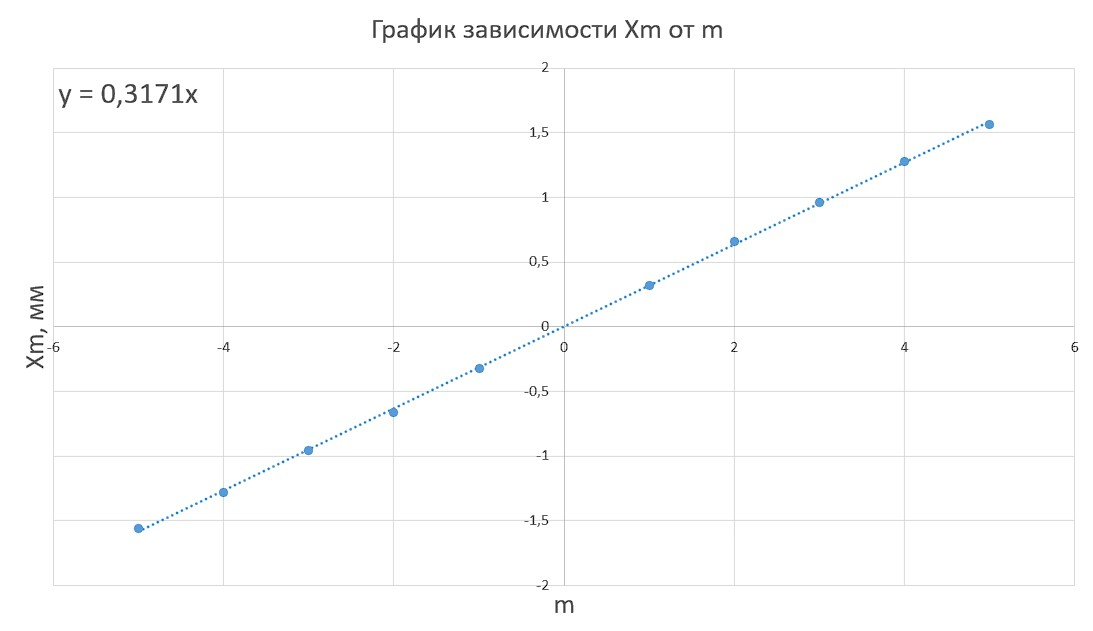
\includegraphics[scale=0.75]{graph2.jpg}
	\label{graph1}
\end{figure}

По углу наклона найдём расстояние между соседними минимумами. Получается $\Delta	X = 0,3171 \pm 0,0019$ мм.

\subsection{Качественные наблюдения}
При смещении S1 не происходит сдвига дифракционной картины. 
Это связано с тем, что картина находится в фокальной плоскости 
линзы S2, куда приходят почти параллельные лучи. При уменьшении 
ширины щели картина растягивается, что согласуется с формулой 
(\ref{xm}).

\subsection{Дифракция Фраунгофера на двух щелях}
Для начала пшсчроаем число светлых промежутков между двумя самыми удалёнными тёмными полосами. Получилось $N = 19$. Зная расстояние между этими двумя полосами, можно найти расстояние между минимумами $\delta x = \frac{X}{N} = 0,050 \pm 0,001$ мм. Посчитаем d по формуле (\ref{dx}). Получается $d = 1,50 \pm 0,03$ мм. Значение находится рядом с измеренным $d = 1,64$ мм.

Первое исчезновение полос наступает при $b_0 = 0,175 \pm 0,002$ мм. Зная это, теперь найдем число полос внутри главного максимума по формуле (\ref{n}). Получается $n = 18,5 \approx 19$(так как число полос должно быть целым), что совпадает с числом посчитанных на опыте тёмных полос. 

Теперь сравним измеренную величину $b_0$ с расчётом по формуле $(12)$. $b = 0,03$ мм, значит изображения нельзя считать различными(т.к. критерий Рэлея не выполняется).


\section{Вывод}
В ходе работы мы изучили два основных типа дифракции: Френеля и 
Фраунгофера при разных размерах щели и провели качественные 
наблюдения этих явлений, а также экспериментально проверили 
справедливость теоретических формул.

Дифракция Френеля: 

Значение для ширины щели, вычисленное по формуле (1), близко к значению, вычисленному при помощи микрометрического винта. Некоторые отличия 
результата от цели можно связать с неточностью определения 
«сдвига» микроскопа и нуля микрометрического винта. 

Дифракция Фраунгофера на одной щели: 
Значение для ширины щели вычисленное по формуле (5), совпадает в пределах погрешности с величиной, измеренной микрометрической шкалой, что подтверждает теоретические выкладки и говорит о выполнении предложенной теории.

Дифракция Фраунгофера на двух щелях:
Значения расстояния между щелями $d$ и числа интерфереционных полос $n$ либо совпадают в пределах погрешности с измеренной величиной(именно такое выполняется для $d$), либо полностью совпадают с измеренным значением(для $n$), что подтверждает правильность выполнения эксперимента и выполнение предложенной теории.


\end{document}